\documentclass{vie16}
\usepackage{wrapfig}
\usepackage{float}
\usepackage{amsmath}
\usepackage[table,xcdraw]{xcolor}
\usepackage{booktabs}
\usepackage{multirow}
\usepackage{adjustbox}

% Path to figures
\graphicspath{{Fig/}}

% Criar fluxogramas
\usepackage[latin1]{inputenc}
\usepackage{tikz}
\usetikzlibrary{shapes,arrows} 

% definindo blocos para o fluxograma
\tikzstyle{decision} = [diamond, draw, fill=blue!20, 
    text width=6.5em, text badly centered, node distance=3cm, inner 
    sep=0pt]
\tikzstyle{decisionmi} = [diamond, draw, fill=blue!20, 
    text width=1.5em, text badly centered, node distance=3cm, inner 
    sep=0pt]
\tikzstyle{block} = [rectangle, draw, fill=blue!20, 
    text width=16em, text centered, rounded corners, minimum height=4em]
\tikzstyle{blockm} = [rectangle, draw, fill=blue!20, 
    text width=6em, text centered, rounded corners, minimum height=4em]
\tikzstyle{blockmg} = [rectangle, draw, fill=blue!20, 
    text width=10em, text centered, rounded corners, minimum height=2em]
\tikzstyle{blockmi} = [rectangle, draw, fill=blue!20, 
    text width=3em, text centered, rounded corners, minimum height=2em]
\tikzstyle{blockf} = [rectangle, draw, fill=blue!20, 
    text width=16em, text centered, rounded corners, minimum height=4em]
\tikzstyle{line} = [draw, -latex']
\tikzstyle{cloud} = [draw, ellipse,fill=red!20, node distance=3cm,
    minimum height=3em]
\tikzstyle{cloudr} = [draw, ellipse,fill=green!20, node distance=3cm,
    minimum height=3em]

\begin{document}
\title{Global optimization for AVO inversion: Analysis of ray theory based 
forward modelling algorithm}
\author{W. C. Ferreira, F. Hilterman, L. A. Diogo, J. Schleicher and H. B. 
Santos}
\maketitle


\begin{abstract}
The Amplitude Variation with Offset (AVO) inversion has been studied in 
order to recover the P-wave, S-wave velocity and density parameters of the 
stratified medium. A global optimization technique was used due to the 
multi parametric behaviour of the AVO inversions which is strongly affected 
by how good is the initial information in model based schemes. An analyse 
to verify the effects of the dependency between P-wave, S-wave velocity 
and density in the recovered parameters was also performed using the 
Gardner and Castagna empirical relations as constrains. However, the 
forward modelling is the main resource consumer in such techniques. The 
genetic algorithm was implemented in FORTRAN 77/90  and a \textit{table 
based} ray theory algorithm was developed in order to allow a large amount 
of models in the global search. Our results show that the genetic algorithm 
was capable to recover the physical parameters with good agreement for the 
examples using the empirical constraints, but was also capable to converge 
to particular solutions which was far from the correct answer, but good 
answers to explain the observed dataset. The forward modelling algorithm 
has shown excellent performance to be used in global optimization schemes 
being able to compute more than 300.000 synthetic seismograms in less 
than 30 minutes.
\end{abstract}

\newpage
\section{Introduction}
The AVO (Amplitude Variation with Offset) anomaly has been widely used in 
the industry as a direct hydrocarbon indicator. However, applications to 
inverse problems has also risen interest in the phenomenon. The 
formulation to compute an estimative of the amplitudes with increasing 
angle (offset) of incidence is classicaly attributed to \cite{Zoeppritz1919} 
and \cite{Knott1899} for plane waves. \cite{Rosa1976} derived and verified 
the ill-posedness of the Zoeppritz equations meaning that we have multiple  
combinations of input to produce the same output.  Moreover, 
\cite{Stoffa1991}, \cite{Mallick1995} and others suggest global optimization 
schemes to treat the AVO inversion due to its multiparametric formulation 
which implies a very complex solution space with many local minima which 
harden the process of finding good solutions. However, the process of 
global optimizations requires many forward modellings which increase 
considerably the time of computation. Many of the works published in 
literature uses forward modelling algorithms based in techniques to solve 
the wave equation, therefore demanding great computational power. This 
project believes that ray theory is enough for many applications in 
exploration seismology and provide an implementation of a forward 
modelling algorithm called \textit{table-based ray theory} in FORTRAN 
77/90 in order to verify its performance and boosts in computations of 
global optimizations. The technique implemented to perform the search in 
the solution space was the genetic algorithm based on findings of 
\cite{Stoffa1991} and \cite{Sen1992} and using the Gardner and Castagna 
empirical relationships as constrains to verify the dependency among the 
parameters.

\section{Synthetic CMP seismogram: forward modelling}
The forward modelling algorithm implemented is the \textit{Table-based ray 
tracing}. The Earth model assumed is the isotropic layer cake model where 
the parametric equation are used to compute the two-way traveltime 
\cite{Slotnick}, the equations are given by

\begin{eqnarray}
x & = & 2\sum_{i=1}^{n} \frac {h_{i}pv_{i}} {(1 -
p^{2}v_{i}^{2})^{1/2}} \ ,\label{eq.x} \\
t & = & 2\sum_{i=1}^{n} \frac {h_{i}} {v_{i}(1 - p^{2}v_{i}^{2})^{1/2}} \ ,
\label{eq.t}
\end{eqnarray}
%
where $h_{i}$, $v_{i}$ and $p$ are, respectively, the thickness of the layers, 
the velocities and the ray parameter which is defined by

\begin{equation}
p = \frac{\sin(\theta_{i})}{v_{i}}\ ,\label{eq.p}
\end{equation}

where $\theta_i$ is the angle between the seismic ray and the vertical in the 
$i$-th layer. Using a sonic log or other vertical velocity information is 
possible to build 4 different tables (\textit{velocity, angle, traveltime, 
offsets} using equations \ref{eq.x}, \ref{eq.t} and the Snell's Law to figure out 
the transmitted angle to the layer below.

To start the process we assign angles varying from 0 to 90 degree in the first 
row of the \textit{angle table} . The step between each cell will also 
determine the accuracy of the modelling. Then, using Snell's Law and the 
velocity of the first layer (first row of velocity table) we compute the 
transmitted angle. In this fashion, recursively, we fill the \textit{angle table}. 
The next step for the synthetic seismogram modelling requires the 
calculation of the reflectivity at each interface. It was used the Shuey's 
approximation \cite{Shuey1985} given by

\begin{equation}
R_{P} (\theta) = A + B\sin^{2}(\theta) + C\sin^{2}(\theta)\tan^{2}(\theta)
\ , \label{eq.shuey}
\end{equation}

where $\theta$ is the incidence angle and the terms $A$, $B$ and $C$ are 
defined as

\begin{equation}
\begin{split}
A & = \frac{1}{2} \left(\frac{\triangle V_{P}}{V_{P}}     +
\frac{\triangle \rho}{\rho}     \right)\ , \\
B & = \frac{1}{2} \frac{\triangle V_{P}}{V_{P}}  - 2\left(\frac{
V_{S}}{V_{P}}\right)^{2}  \left(\frac{2\triangle V_{S}}{V_{S}} +
\frac{\triangle \rho}{\rho}\right)   \ , \\
C & = \frac{1}{2} \left(\frac{\triangle V_{P}}{V_{P}} \right) \ .
\end{split}
\end{equation}

where in these expressions, $\triangle V_{P} = V_{P2} - V_{P1}$, $\triangle 
V_{S} = V_{S2} - V_{S1}$, $\triangle \rho = \rho_{2} - \rho_{1}$, where 
$V_{P}$, $V_{S}$ e $\rho$ are arithmetic averages from P-wave, S-wave 
velocities and the density.

Finally in order to build the CMP synthetic seismogram we define which are 
the offsets to model and start a search row-by-row inside the \textit{offset 
table} looking for the requested offsets. Once the value is found, we go into 
the same cell position inside the \textit{angle table}, \textit{traveltime table} 
and \textit{reflectivity table} to place the reflection coefficient from that 
position in the correct time arrival inside the trace.

The algorithm is simple and provide the opportunity to be easily adapted to 
study more complex effects such as the stretching in NMO correction, NMO 
without stretch (Raytrace NMO correction), array effects which affect the 
amplitude of the wave received by the streamer, easily extraction of AVO 
attributes, polar anisotropic media, etc.
 
\section{Global optimization approach: Genetic Algorithm}
\begin{wrapfigure}{l}{0.5\textwidth}
 \centering
 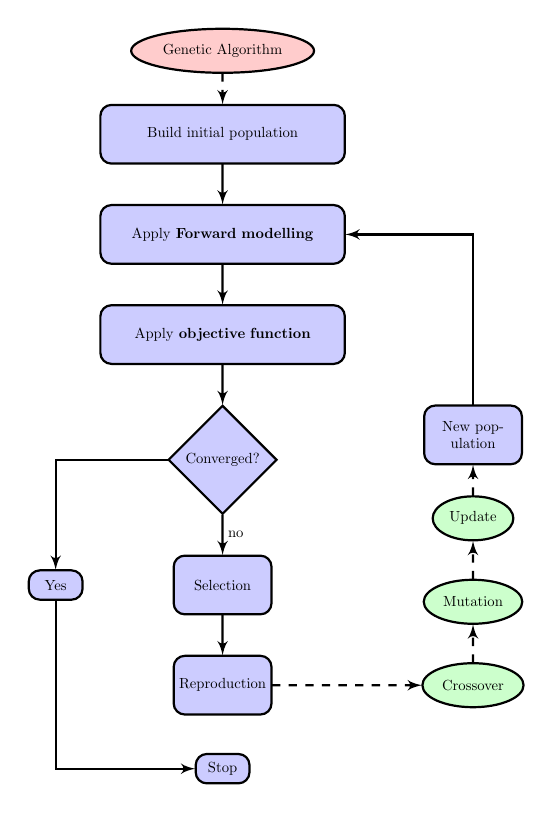
\begin{tikzpicture}[thick,scale=0.53, every 
 node/.style={scale=0.53},node distance = 2.4cm, auto]
    % Place nodes
    \node [block] (init) {Build initial population};
    \node [cloud, above of=init, node distance=2cm] (expert) {Genetic 
    Algorithm};
    \node [block, below of=init] (identify) {Apply \textbf{Forward modelling}};
    \node [blockf, below of=identify] (pop) {Apply \textbf{objective 
    function}}; 
    \node [decision, below of=pop] (evaluate) {Converged?};
    \node [blockm, below of=evaluate, node distance=3cm] (select) 
    {Selection};
    \node [blockm, below of=select] (reprod) {Reproduction};
    \node [cloudr, right of=reprod, node distance=6cm] (crossover) 
    {Crossover};
    \node [cloudr, above of=crossover, node distance=2cm] (mutation) 
    {Mutation};
    \node [cloudr, above of=mutation, node distance=2cm] (update) {Update};
    \node [blockm, above of=update, node distance=2cm] (newpop) {New 
    population};
    \node [blockmi, below of=reprod, node distance=2cm] (stop) {Stop};
    \node [blockmi, left of=select, node distance=4cm] (sim) {Yes};

    % Draw edges
    \path [line] (init) -- (identify);
    \path [line] (identify) -- (pop);
    \path [line] (pop) -- (evaluate);
    \path [line,dashed] (expert) -- (init);
    \path [line] (evaluate) --  node {no} (select);
    \path [line] (select) -- (reprod);
    \path [line,dashed] (reprod) -- (crossover);
    \path [line, dashed] (crossover) -- (mutation);
    \path [line, dashed] (mutation) -- (update);
    \path [line, dashed] (update) -- (newpop);  
    \path [line] (newpop) |- (identify);
    \path [line] (evaluate) -| (sim);
    \path [line] (sim) |- (stop);
  
\end{tikzpicture}
\caption{Flowchart of the genetic algorithm implemented in FORTRAN 
77/90.}\label{fig.fluxo}
\end{wrapfigure}

The genetic algorithm (Figure 1) is a technique used to perform global 
optimizations based in the natural selection \cite{Holland1975}. In order to 
simulate this process, the algorithm constantly modify the initial 
pseudo-random population in order to reach local minima positions. 
Initially each member of the pseudo-random population is a potential 
solution to the problem and after some iterations the genetic algorithm will 
guide the population to the best fit positions.

The algorithm needs to \textit{select} a percentage of the population to start 
the reproduction scheme where the \textit{crossover} and the 
\textit{mutation} are the two classic tecniques to exchange genetic 
information between the members and also randomly change the genetic 
information to provide exploration of the solution space. In order to select 
the members of the population we need to measure the fitness between each 
potential solution and the data we want to optimize. The objective function 
used was proposed by \cite{Porsani2000} and is given by

\begin{equation}
h = \frac{2y^{T} x} {y^{T}y + x^{T}x} \label{eq.Porsani}
\end{equation} 

where, $x$ e $y$ are respectively the observed data and modelled data in 
the time domain and  $x^{T}$, $y^{T}$ are their transposes. In order to 
constrain the inverse problem due to the dependency between S-wave 
velocity and density with P-wave velocity, it was used the Gardner 
\citep{Gardner01121974} and Castagna \citep{Castagna01041985} relations 
to write S-wave and density as a function of P-wave.

\section{Results}
A synthetic model was used in order to verify the global optimization 
method for AVO inversion and its relationships with the prior informations 
(Gardner and Castagna constrains) and also to analyse the performance of 
the forward modelling algorithm proposed. The physical parameters for the 
synthetic model is described in the Table 1. The thickness between the two 
inner layers was chosen to be small enough to allow interaction between the 
wavelets.

\begin{wraptable}{l}{0.5\textwidth}
\caption{eee}
\begin{adjustbox}{max width=0.46\textwidth}
\label{model}
\begin{tabular}{@{}|
>{\columncolor[HTML]{9B9B9B}}c |cccc@{}}
\toprule
\textbf{Layers} & \multicolumn{1}{c|}{\cellcolor[HTML]{9B9B9B}\textbf{\begin{tabular}[c]{@{}c@{}}Thickness\\ (meters)\end{tabular}}} & \multicolumn{1}{c|}{\cellcolor[HTML]{9B9B9B}\textbf{\begin{tabular}[c]{@{}c@{}}Vp \\ (m/s)\end{tabular}}} & \multicolumn{1}{c|}{\cellcolor[HTML]{9B9B9B}\textbf{\begin{tabular}[c]{@{}c@{}}Vs\\ (m/s)\end{tabular}}} & \multicolumn{1}{c|}{\cellcolor[HTML]{9B9B9B}\textbf{\begin{tabular}[c]{@{}c@{}}Density\\ (g/cc)\end{tabular}}} \\ \midrule
1               & 1000                                                                                                               & 2000                                                                                                      & 551.72                                                                                                   & 1.5381                                                                                                         \\ \cmidrule(r){1-1}
2               & 50                                                                                                                 & 2800                                                                                                      & 1241.38                                                                                                  & 1.6731                                                                                                         \\ \cmidrule(r){1-1}
3               & 50                                                                                                                 & 2300                                                                                                      & 810.34                                                                                                   & 1.5928                                                                                                         \\ \cmidrule(r){1-1}
4               & 500                                                                                                                & 3000                                                                                                      & 1413.80                                                                                                  & 1.7022                                                                                                         \\ \bottomrule
\end{tabular}
\end{adjustbox}
\end{wraptable}

The parameters used in the forward modelling shown in Figure 1 was a zero 
phase Ricker wavelet with central frequency in 40Hz and discretization time 
of 2ms. In order to perform the global optimization the CMP gathers have to 
be previously corrected from the \textit{normal moveout}.
\\
The parameters used in the \textit{genetic algorithm} is given by 
\textit{selection rate} of $50\%$, $P_{mutation}$ = 0.1, $P_{update}$ = 
0.47, $P_{crossover}$ = 0.90, 1000 members in the population and a 
convergence criterion of 200 iterations.

In the following results only the parameters from the fourth layer of the 
model from Table \ref{model} will be shown in more detail due to the limit 
of space. The Figure 2 shows the evolution of the genetic algorithm 
solutions for the P-wave velocity parameter in the fourth layer when 
running with and without the Gardner and Castagna constrains. As we can 
see in Figure 2(a), after few iterations the algorithm is already guiding all the 
members in the population close to the correct position in the solution 
space.

However, the Figure 2(b) shows that even with the lack of additional 
constrains to restrict the solutions, the algorithm is leading the population 
to particular solutions which are not so close to the correct one but are 
good answers to the inverse problem as we can see in Table 2.

\begin{figure}[H]
\centering
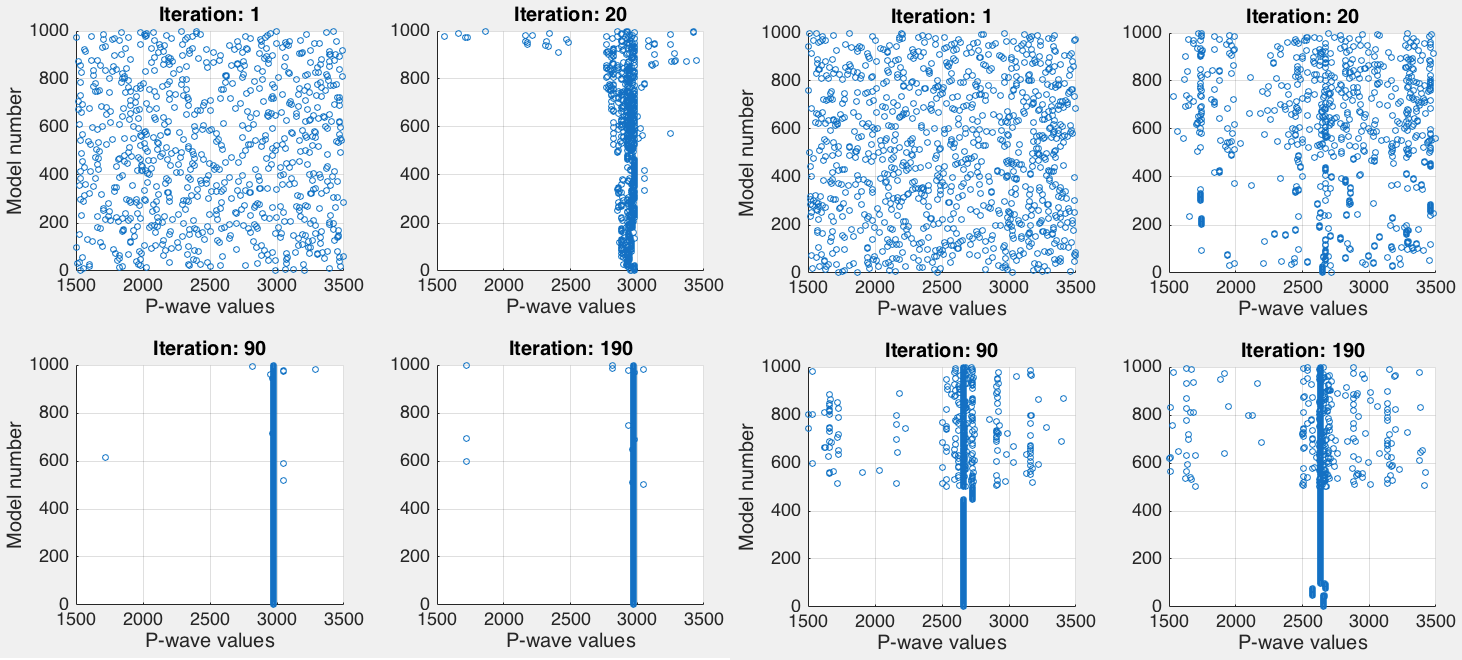
\includegraphics[scale=0.32]{iterations_vp4_refeita}
   \caption{testE}
\end{figure}

In Table 2 we can see the values for the best model recovered with and 
without the constrains in the parameters. The algorithm performed 301.000 
forward modelling in 36 minutes. Even with more than $20\%$ of relative 
error in average, the best model recovered without the constrains still 
produce a very similar CMP gather as we can verify by the correlation 
coefficient value.


\begin{table}[h!]
\caption{My caption}
\begin{adjustbox}{max width=\textwidth}
\label{my-label}
\begin{tabular}{@{}|c|ccccc@{}}
\toprule
\rowcolor[HTML]{C0C0C0} 
\textbf{Parameters}                                                                                & \multicolumn{1}{c|}{\cellcolor[HTML]{C0C0C0}\textbf{Synthetic Model}} & \multicolumn{2}{c|}{\cellcolor[HTML]{C0C0C0}\textbf{\begin{tabular}[c]{@{}c@{}}Recovered Model\\ (with constrains)\end{tabular}}}                                                             & \multicolumn{2}{c|}{\cellcolor[HTML]{C0C0C0}\textbf{\begin{tabular}[c]{@{}c@{}}Recovered Model\\ (without constrains)\end{tabular}}}                                                         \\ \midrule
\rowcolor[HTML]{C0C0C0} 
                                                                                                   & \multicolumn{1}{c|}{\cellcolor[HTML]{C0C0C0}}                         & \multicolumn{1}{c|}{\cellcolor[HTML]{C0C0C0}\textbf{Parameters}} & \multicolumn{1}{c|}{\cellcolor[HTML]{C0C0C0}\textbf{\begin{tabular}[c]{@{}c@{}}Relative Percentual \\ Error\end{tabular}}} & \multicolumn{1}{c|}{\cellcolor[HTML]{C0C0C0}\textbf{Parameters}} & \multicolumn{1}{c|}{\cellcolor[HTML]{C0C0C0}\textbf{\begin{tabular}[c]{@{}c@{}}Relative Percentual\\ Error\end{tabular}}} \\ \midrule
\cellcolor[HTML]{C0C0C0}                                                                           & \cellcolor[HTML]{FFFFC7}2000                                          & \cellcolor[HTML]{9AFF99}2000                                     & \cellcolor[HTML]{9AFF99}0.00                                                                                               & \cellcolor[HTML]{BBDAFF}2002                                     & \cellcolor[HTML]{BBDAFF}-0.10                                                                                             \\
\cellcolor[HTML]{C0C0C0}                                                                           & \cellcolor[HTML]{FFFFC7}2800                                          & \cellcolor[HTML]{9AFF99}2788                                     & \cellcolor[HTML]{9AFF99}0.43                                                                                               & \cellcolor[HTML]{BBDAFF}2699                                     & \cellcolor[HTML]{BBDAFF}3.61                                                                                              \\
\cellcolor[HTML]{C0C0C0}                                                                           & \cellcolor[HTML]{FFFFC7}2300                                          & \cellcolor[HTML]{9AFF99}2280                                     & \cellcolor[HTML]{9AFF99}0.87                                                                                               & \cellcolor[HTML]{BBDAFF}2394                                     & \cellcolor[HTML]{BBDAFF}-4.09                                                                                             \\
\multirow{-4}{*}{\cellcolor[HTML]{C0C0C0}\begin{tabular}[c]{@{}c@{}}P-wave\\ (m/s)\end{tabular}}   & \cellcolor[HTML]{FFFFC7}3000                                          & \cellcolor[HTML]{9AFF99}2971                                     & \cellcolor[HTML]{9AFF99}0.97                                                                                               & \cellcolor[HTML]{BBDAFF}2658                                     & \cellcolor[HTML]{BBDAFF}11.40                                                                                             \\ \midrule
\cellcolor[HTML]{C0C0C0}                                                                           & \cellcolor[HTML]{FFFFC7}551.72                                        & \cellcolor[HTML]{9AFF99}552.71                                   & \cellcolor[HTML]{9AFF99}-0.07                                                                                              & \cellcolor[HTML]{BBDAFF}778                                      & \cellcolor[HTML]{BBDAFF}-41.01                                                                                            \\
\cellcolor[HTML]{C0C0C0}                                                                           & \cellcolor[HTML]{FFFFC7}1241.38                                       & \cellcolor[HTML]{9AFF99}1231                                     & \cellcolor[HTML]{9AFF99}0.84                                                                                               & \cellcolor[HTML]{BBDAFF}1327                                     & \cellcolor[HTML]{BBDAFF}-6.90                                                                                             \\
\cellcolor[HTML]{C0C0C0}                                                                           & \cellcolor[HTML]{FFFFC7}810.34                                        & \cellcolor[HTML]{9AFF99}793                                      & \cellcolor[HTML]{9AFF99}2.14                                                                                               & \cellcolor[HTML]{BBDAFF}1106                                     & \cellcolor[HTML]{BBDAFF}-36.49                                                                                            \\
\multirow{-4}{*}{\cellcolor[HTML]{C0C0C0}\begin{tabular}[c]{@{}c@{}}S-wave\\ (m/s)\end{tabular}}   & \cellcolor[HTML]{FFFFC7}1413                                          & \cellcolor[HTML]{9AFF99}1389                                     & \cellcolor[HTML]{9AFF99}1.75                                                                                               & \cellcolor[HTML]{BBDAFF}1358                                     & \cellcolor[HTML]{BBDAFF}3.95                                                                                              \\ \cmidrule(r){1-1}
\cellcolor[HTML]{C0C0C0}                                                                           & \cellcolor[HTML]{FFFFC7}1.5381                                        & \cellcolor[HTML]{9AFF99}1.538                                    & \cellcolor[HTML]{9AFF99}0.01                                                                                               & \cellcolor[HTML]{BBDAFF}1.1408                                   & \cellcolor[HTML]{BBDAFF}25.83                                                                                             \\
\cellcolor[HTML]{C0C0C0}                                                                           & \cellcolor[HTML]{FFFFC7}1.6731                                        & \cellcolor[HTML]{9AFF99}1.671                                    & \cellcolor[HTML]{9AFF99}0.13                                                                                               & \cellcolor[HTML]{BBDAFF}1.2932                                   & \cellcolor[HTML]{BBDAFF}22.71                                                                                             \\
\cellcolor[HTML]{C0C0C0}                                                                           & \cellcolor[HTML]{FFFFC7}1.5928                                        & \cellcolor[HTML]{9AFF99}1.589                                    & \cellcolor[HTML]{9AFF99}0.24                                                                                               & \cellcolor[HTML]{BBDAFF}1.1466                                   & \cellcolor[HTML]{BBDAFF}28.01                                                                                             \\
\multirow{-4}{*}{\cellcolor[HTML]{C0C0C0}\begin{tabular}[c]{@{}c@{}}Density\\ (g/cc)\end{tabular}} & \cellcolor[HTML]{FFFFC7}1.7022                                        & \cellcolor[HTML]{9AFF99}1.698                                    & \cellcolor[HTML]{9AFF99}0.25                                                                                               & \cellcolor[HTML]{BBDAFF}1.4416                                   & \cellcolor[HTML]{BBDAFF}15.31                                                                                             \\ \midrule
\multicolumn{1}{|l|}{\cellcolor[HTML]{C0C0C0}Correlation Coef.}                                    & \multicolumn{1}{c|}{1}                                                & \multicolumn{2}{c|}{0.999887645}                                                                                                                                                              & \multicolumn{2}{c|}{0.999847412}                                                                                                                                                             \\ \bottomrule
\end{tabular}
\end{adjustbox}
\end{table}


\section{Conclusions}
The forward modelling algorithm presented has shown excellent potential to 
be used in global optimization schemes by providing good performance in a 
regular computer. The constrains are also helpful in the process however the 
result without constrains indicate that we can still converge to particular 
results. The genetic algorithm will be formulated inside the Bayesian 
framework to provide solid statistical informations about the distribution of 
the solutions during the iterations. It's expected to be able to visualize 
distinguishable concentration of particular solutions which could be useful 
to determine possible scenarios for the recovered parameters. Finally, for 
future work in this project will also introduce errors in the models and an 
application to real data to verify the reliability of this technique.



\section{Acknowledgements}

Valeu Henrique. rsrs

\bibliography{lib}
\end{document} 